\newpage
\chapter*{Anhang}
\label{cha:anhang}
\addcontentsline{toc}{chapter}{Anhang}

\section*{Anhang 1}
\label{sec:anhang-1}

\begin{figure}[ht]
\begin{center}
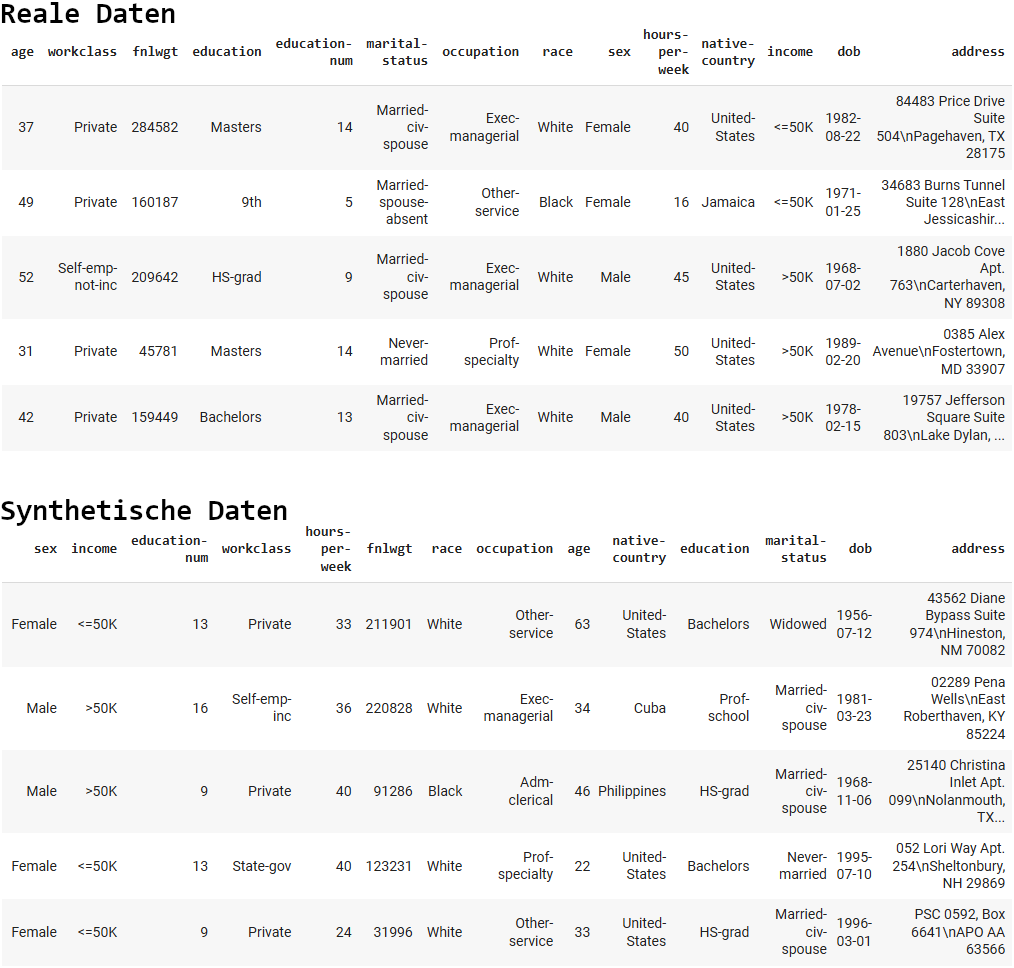
\includegraphics[width=\textwidth]{img/real-vs-synthetic-data.png}
\caption[Gegenüberstellung realer und synthetischer Daten]{Gegenüberstellung realer und synthetischer Daten\footnotemark}
\label{fig:real-vs-synthetic}
\end{center}
\end{figure}
\footnotetext{Eigene Darstellung}

\newpage
\section*{Anhang 2}
\label{sec:anhang-2}

\inputminted{python}{lst/sdv.py}
\captionof{listing}{Python-Implementierung zur Erstellung synthetischer Zensusdaten}